
\section{Biểu diễn thông tin}

Ta đã xem xét các kỹ thuật để lưu trữ các bít, bây giờ ta sẽ xem xét cách mã hoá thông tin
như dãy bít. Ta sẽ quan tâm đến các phương pháp phổ biến để mã hoá văn bản, dữ liệu số,
hình ảnh, âm thanh. [....]

\subsection*{Biểu diễn văn bản}
Thông tin của văn bản thường được biểu diễn bởi mã của các ký hiệu trong nó (như các chữ
cái trong một bảng chữ, các dấu chấm, phảy,...). Từ đó, văn bản được biểu diễn như một xâu
bít dài trong đó dãy bít liên tiếp biểu diễn các ký hiệu liên tiếp trong văn bản gốc.

Trong những năm~$1940$ và~$1950$, nhiều kiểu mã như vậy đã được thiết kế và được sử dụng
trong liên lạc giữa các thành phần khác nhau của thiết bị, điều này cũng dẫn đến phức tạp
trong truyền thông. Để làm giảm những phức tạp này, \textbf{Hội Chuẩn Quốc Gia Hoa Kỳ
  (ANSI)} đã chọn Mã chuẩn của Mỹ để trao đổi thông tin (\textbf{American Standard Code
  for Information Interchange (ASCII)}). Mã này dùng các xâu bảy bít để biểu diễn các chữ
cái hoa và chữ cái thường của bảng chữ Tiếng Anh, ký hiệu dấu, các số từ $0$ tới $9$, và
một số thông tin điều khiển như ký hiệu xuống dòng, ký hiệu trở về, và tab. Ngày nay, mã
ASCII được mở rộng sang thành dạng tám bít bằng cách thêm một $0$ vào bít trái nhất của
xâu bảy bít. Kỹ thuật này không chỉ cho ta một mã phù hợp với kích thước ô nhớ theo byte
mà còn cho ta thêm $128$ bít nữa (những mã bắt đầu bởi $1$) là những ký hiệu mở rộng thêm
từ bảng mã ASCII ban đầu. Không may, mỗi nhà sản xuất hướng sử dụng các ký hiệu được mở
rộng theo cách riêng của họ, nên dữ liệu mà các xâu bít này biểu diễn không dễ chuyển từ
các ứng dụng của nhà sản xuất này sang ứng dụng của nhà sản suất khác.

Một phần của ASCII theo định dạng xâu tám bít cho mỗi ký hiệu được chỉ ra bởi Phụ lục
\ref{}. Bằng cách tra phụ lục này, ta có thể giải mã xâu bít Hình~\ref{fig:fig1.13}
như thông điệp ``Hello.''.

\begin{figure}[bt]
\centering
\begin{tabular}{cccccc}
  $\underbrace{01001000}$ & $\underbrace{01100101}$
  & $\underbrace{01101100}$ & $\underbrace{01101100}$  
  & $\underbrace{01101111}$ & $\underbrace{00101110}$ \\
  \texttt{H}  & \texttt{e}  & \texttt{l} & \texttt{l} & \texttt{o}
  & \texttt{.}                                        \\
\end{tabular}
\caption{Thông điệp ``Hello.'' biểu diễn ở ASCII}
  \label{fig:fig1.13}
\end{figure}

Mặc dù bảng mã ASCII đã được thừa nhận rộng rãi trong nhiều năm, tuy nhiên do nhu cầu trình
bày tài liệu trong nhiều ngôn ngữ, những mã khác mở rộng hơn hiện nay lại trở nên phổ
biến. Một trong số đó là \textbf{Unicode}, đã được phát triển nhờ hợp tác của một vài nhà
sản xuất phần cứng hàng đầu và nhanh chóng nhận được sự ủng hộ của cộng đồng quốc tế. Mã
này dùng một xâu $16$ bít duy nhất để biểu biễn một ký hiệu. Vậy, Unicode bao gồm $65,536$
xâu bít khác nhau--đủ để biểu diễn các văn bản ở nhiều ngôn ngữ như Tiếng Trung, Tiếng
Nhật, và Tiếng Do Thái.

Chuẩn hoá cho một bộ mã đầy đủ Unicode được phát triển bởi \textbf{Tổ chức Quốc Tế về
  Chuẩn hoá} (International Organization for Standardization, viết tắt là
\textbf{ISO}). Mã này dùng các xâu độ dài $32$ bít, và có khả năng biểu diễn hàng tỉ ký
hiệu khác nhau.

Một file bao gồm một dãy ký hiệu dài được mã hoá dùng ASCII hoặc Unicode thường được gọi
là một \textbf{file văn bản}. Một ý quan trọng mà ta phải phân biệt, đó là giữa một file
văn bản đơn giản có thể thao tác bởi các chương trình công cụ được gọi là \textbf{trình
  soạn thảo} và các file phức tạp hơn được tạo bởi \textbf{bộ xử lý văn bản}. Cả hai đều
bao gồm các văn bản. Tuy nhiên, một file văn bản chỉ chứa các ký hiệu mã hoá của văn bản,
trong khi đó một file tạo bởi bộ xử lý văn bản chứa nhiều mã riêng biểu diễn các font, các
thông tin về cách gióng hàng,... Hơn nữa, bộ xử lý văn bản có thể sử dụng các mã riêng
thay vì chuẩn ASCII hoặc Unicode để biểu diễn văn bản.

\subsection*{Biểu diễn giá trị số}

Lưu trữ thông tin theo cách mã hoá các ký tự là không hiệu quả khi thông tin là các giá
trị số. Để thấy lý do tại sao, ta cùng xem xét vấn đề lưu trữ giá trị $25$. Nếu ta nhất
định lưu trữ nó như các ký hiệu ở dạng ASCII dùng mỗi byte cho mỗi ký hiệu, ta cần $16$
bít để lưu trữ. Hơn nữa, số lớn nhất ta có thể lưu trữ dùng $16$ bít là $99$. Tuy nhiên,
nếu dùng \textbf{ký hiệu nhị phân} thì với $16$ bít ta có thể lưu trữ mọi số nguyên từ $0$
tới $65,535$. Bởi vậy, ký hiệu nhị phân (hay các dạng khác của nó) được sử dụng rộng rãi
cho việc mã hoá dữ liệu số trên máy tính.

Ký hiệu nhị phân là một cách biểu diễn các giá trị số chỉ dùng các số $0$ và $1$ thay vì
các số $0, 1, 2 , 3, 4, 5, 6, 7, 8, $ và $9$ như trong chữ số truyền thống, hoặc cơ sở
$10$. ta sẽ nghiên cứu hệ thống số đầy đủ trong Mục \ref{}. Bây giờ, ta sẽ chỉ cần một vài
kiến thức cơ sở để hiểu hệ thống này. Với mục đích này, ta sẽ xem xét đồng hồ đo số km
trong các ôtô kiểu cũ [.....]

Do tính hiệu quả này, các thông tin dạng số thường được lưu trữ bởi một dạng ký hiệu nhị
phân thay vì dạng ký hiệu được mã hoá. Ta nói ``một dạng ký hiệu nhị phân'' bởi vì hệ
thống nhị phân được mô tả trực tiếp chỉ là cơ sở cho một vài kỹ thuật lưu trữ số được sử
dụng bên trong máy. Một vài dạng khác của hệ thống nhị phân sẽ được thảo luận sau này. Bây
giờ, ta thuần tuý chỉ để ý rằng hệ thống được gọi là ký hiệu \textbf{bù hai} (xem Phần
\ref{}) là cách chung để lưu trữ các số bởi vì nó cho ta phương pháp thích hợp để biểu
diễn số ấm cũng như số nguyên dương. Để biểu diễn phân số như $4\frac{1}{2}$ hoặc
$\frac{3}{4}$, được gọi là ký hiệu \textbf{dấu chấm động} (xem Mục \ref{}).

\subsection*{Biểu diễn hình ảnh}

Các ứng dụng máy tính ngày nay bao gồm nhiều hơn là chỉ có văn bản và giá trị số. Chúng
còn bao gồm cả hình ảnh, âm thanh, và video. Kỹ thuật phổ biến để biểu diễn ảnh bao gồm
hai loại: \textbf{các kỹ thuật bitmap} và \textbf{các kỹ thuật vectors}. Với kỹ thuật bit
map, một ảnh được biểu diễn như một tập các điểm, mỗi điểm gọi là một \textbf{pixel}, viết
tắt của từ ``picture element.'' (phần tử ảnh). Một ảnh đen trắng được mã hoá như một xâu
bít dài biểu diễn các dòng pixel trong ảnh, trong đó mỗi bít hoặc là bằng $1$ hoặc
bằng~$0$ phụ thuộc khi nào pixel tương ứng là đen hay trắng. Kỹ thuật này được sử dụng
trong hầu hết các máy sao chép (facsimile).

Thuật ngữ \textit{bit map} bắt nguồn từ sự kiện rằng các bít biểu diễn một ảnh theo định
dạng một-bít-cho-một-pixel [...]. Ngày nay thuật ngữ đã được tổng quát hoá để bao gồm mọi
hệ thống trong đó các ảnh được mã hoá theo cách pixel-cạnh-pixel. Ví dụ, trong trường hợp
ảnh đen trắng, mỗi pixel được biểu diễn bởi một tập các bít (thường là tám), cho phép bóng
xám được biểu diễn.

Cách tiếp cận bip map được mở rộng cho ảnh màu, trong đó mỗi điểm ảnh (pixel) được biểu
diễn bởi một tổ hợp các bít chỉ ra có mặt của pixel. Hai cách tiếp cận này là chung. Trong
đó, cách ta sẽ gọi là mã hoá RGB, mỗi điểm ảnh được biểu diễn bởi thành phần màu-- đỏ
(red), xanh lá cây (green) và xanh lam (blue)--tương ứng với ba màu của ánh sáng. Thông
thường ta dùng một byte để biểu diễn cường độ của mỗi thành phần màu. Bởi vậy, mỗi điểm
ảnh cần ba byte để lưu trữ.

Một lựa chọn phổ biến khác để mã hoá RGB là sử dụng thành phần ``độ sáng'' kết hợp với hai
thành phần màu. Ở đây, thành phần ``độ sáng'' được gọi là độ chiếu sáng của điểm ảnh, về
cơ bản nó là tổng của ba thành phần đỏ, xanh lá cây và xanh lam. (Trên thực tế, nó chính
là tổng số ánh sáng trắng trong điểm ảnh, nhưng ở đây ta sẽ không cần quan tâm chi tiết.)
Hai thành phần còn lại được gọi là độ màu xanh lam và độ màu đỏ. Độ màu xanh lam (tương
ứng, độ màu đỏ) được xác định bằng cách tính chênh lệch giữa độ chiếu sáng của điểm ảnh và
tổng số ánh sáng xanh lam (tương ứng tổng số ánh sáng đỏ) trong điểm ảnh. Kết hợp cả ba
thành phần này lại ta được thông tin xác định điểm ảnh.

Tính phổ biến của mã hoá ảnh dùng độ sáng và các thành phần màu bắt nguồn từ lĩnh vực
truyền hình màu bởi vì cách tiếp cận này cho phép tương thích giữa việc mã hoá các ảnh màu
và các tín hiệu nhận được của các tivi đen trắng đời cũ. Thực ra, các ảnh xám có thể được
xem như ảnh màu khi giới hạn chỉ dùng thành phần độ sáng.

Một điểm bất lợi của kỹ thuật bitmap là ảnh không thể thay đổi kích thước một cách tuỳ
ý. Về cơ bản, chỉ có cách phóng to ảnh là tăng độ lớn của điểm ảnh, nhưng nó sẽ làm vỡ
ảnh. (Đây là kỹ thuật dùng trong các camera số gọi là ``digital zoom'', ngược lại với
``optical zoom'' là điều chỉnh thấu kính của cameras.) Kỹ thuật vector cho phép khắc phục
vấn đề này. Với cách tiếp cận này, một ảnh được biểu diễn như một tập các đường thẳng và
đường cong. Kiểu mô tả này bỏ qua chi tiết xem làm thế nào các đường thẳng và đường cong
được vẽ ra thiết bị tạo ảnh mà thay vào đó nó nhấn mạnh đến cách tạo ra một mẫu điểm ảnh
đặc biệt.

Nhiều font trong các hệ thống xử lý văn bản ngày nay được mã hoá dùng kỹ thuật vector. Kỹ
thuật này cho phép làm thay đổi kích thước của ký tự trong văn bản một cách mềm dẻo. Các
font này được gọi là \textbf{scalable fonts}. Ví dụ, TrueType (được phát triển bởi
Microsoft và Apple Computer) là một hệ thống mô tả cách các ký hiệu trong văn bản được
vẽ. Tương tự, PostScript (được phát triển bởi Adobe System) cho phép mô tả các ký tự cũng
như các dữ liệu ảnh tổng quát hơn. Các kỹ thuật biểu diễn vector cũng phổ biến trong các
hệ thống \textbf{thiết kế với trợ giúp của máy tính} (Computer-aided design) trong đó việc
vẽ các đối tượng ba chiều được hiện và được thao tác trên màn hình máy tính.

\subsection*{Biểu diễn âm thanh}

Phương pháp chung nhất để mã hoá thông tin audio để lưu trữ và xử lý trong máy tính là lấy
mẫu biên độ của sóng âm theo từng khoảng và ghi lại như dãy giá trị. Ví dụ, dãy $0$,
$1.5$, $2.0$, $3.0$, $4.0$, $3.0$, $0$ là dãy sóng âm theo biên độ, nói một cách ngắn gọn,
sóng này tăng dần rồi quay lại $0$ (Hình \ref{fig:fig1.14}). Kỹ thuật này sử dụng một tỷ lệ lấy mẫu
là $8000$ mẫu mỗi giây, đã được dùng trong nhiều năm để truyền thông điện thoại khoảng
cách xa. Giọng nói được mã hoá bằng giá trị số biểu diễn biên độ của giọng $8000$ lần
trong một giây. Các giá trị này được truyền đến nơi nhận, tại đây âm của giọng được tái
tạo lại.


Dù tỷ lệ $8000$ mẫu trên giây có vẻ khá nhanh, nhưng nó vẫn không đủ để thu âm với độ
trung thực cao. Để đạt được chất lượng âm thanh cao của đĩa CD nhạc, một tỷ lệ mẫu
$44,100$ mẫu trên giây được dùng. Dữ liệu đạt được từ mỗi mẫu được biểu diễn bởi $16$ bít
($32$ bít cho thu âm stereo). Vậy nên ta cần hơn một triệu bít cho mỗi giây của âm nhạc
thu ở dạng stereo.

\begin{figure}[tbh]
\centering
    \scalebox{0.65}{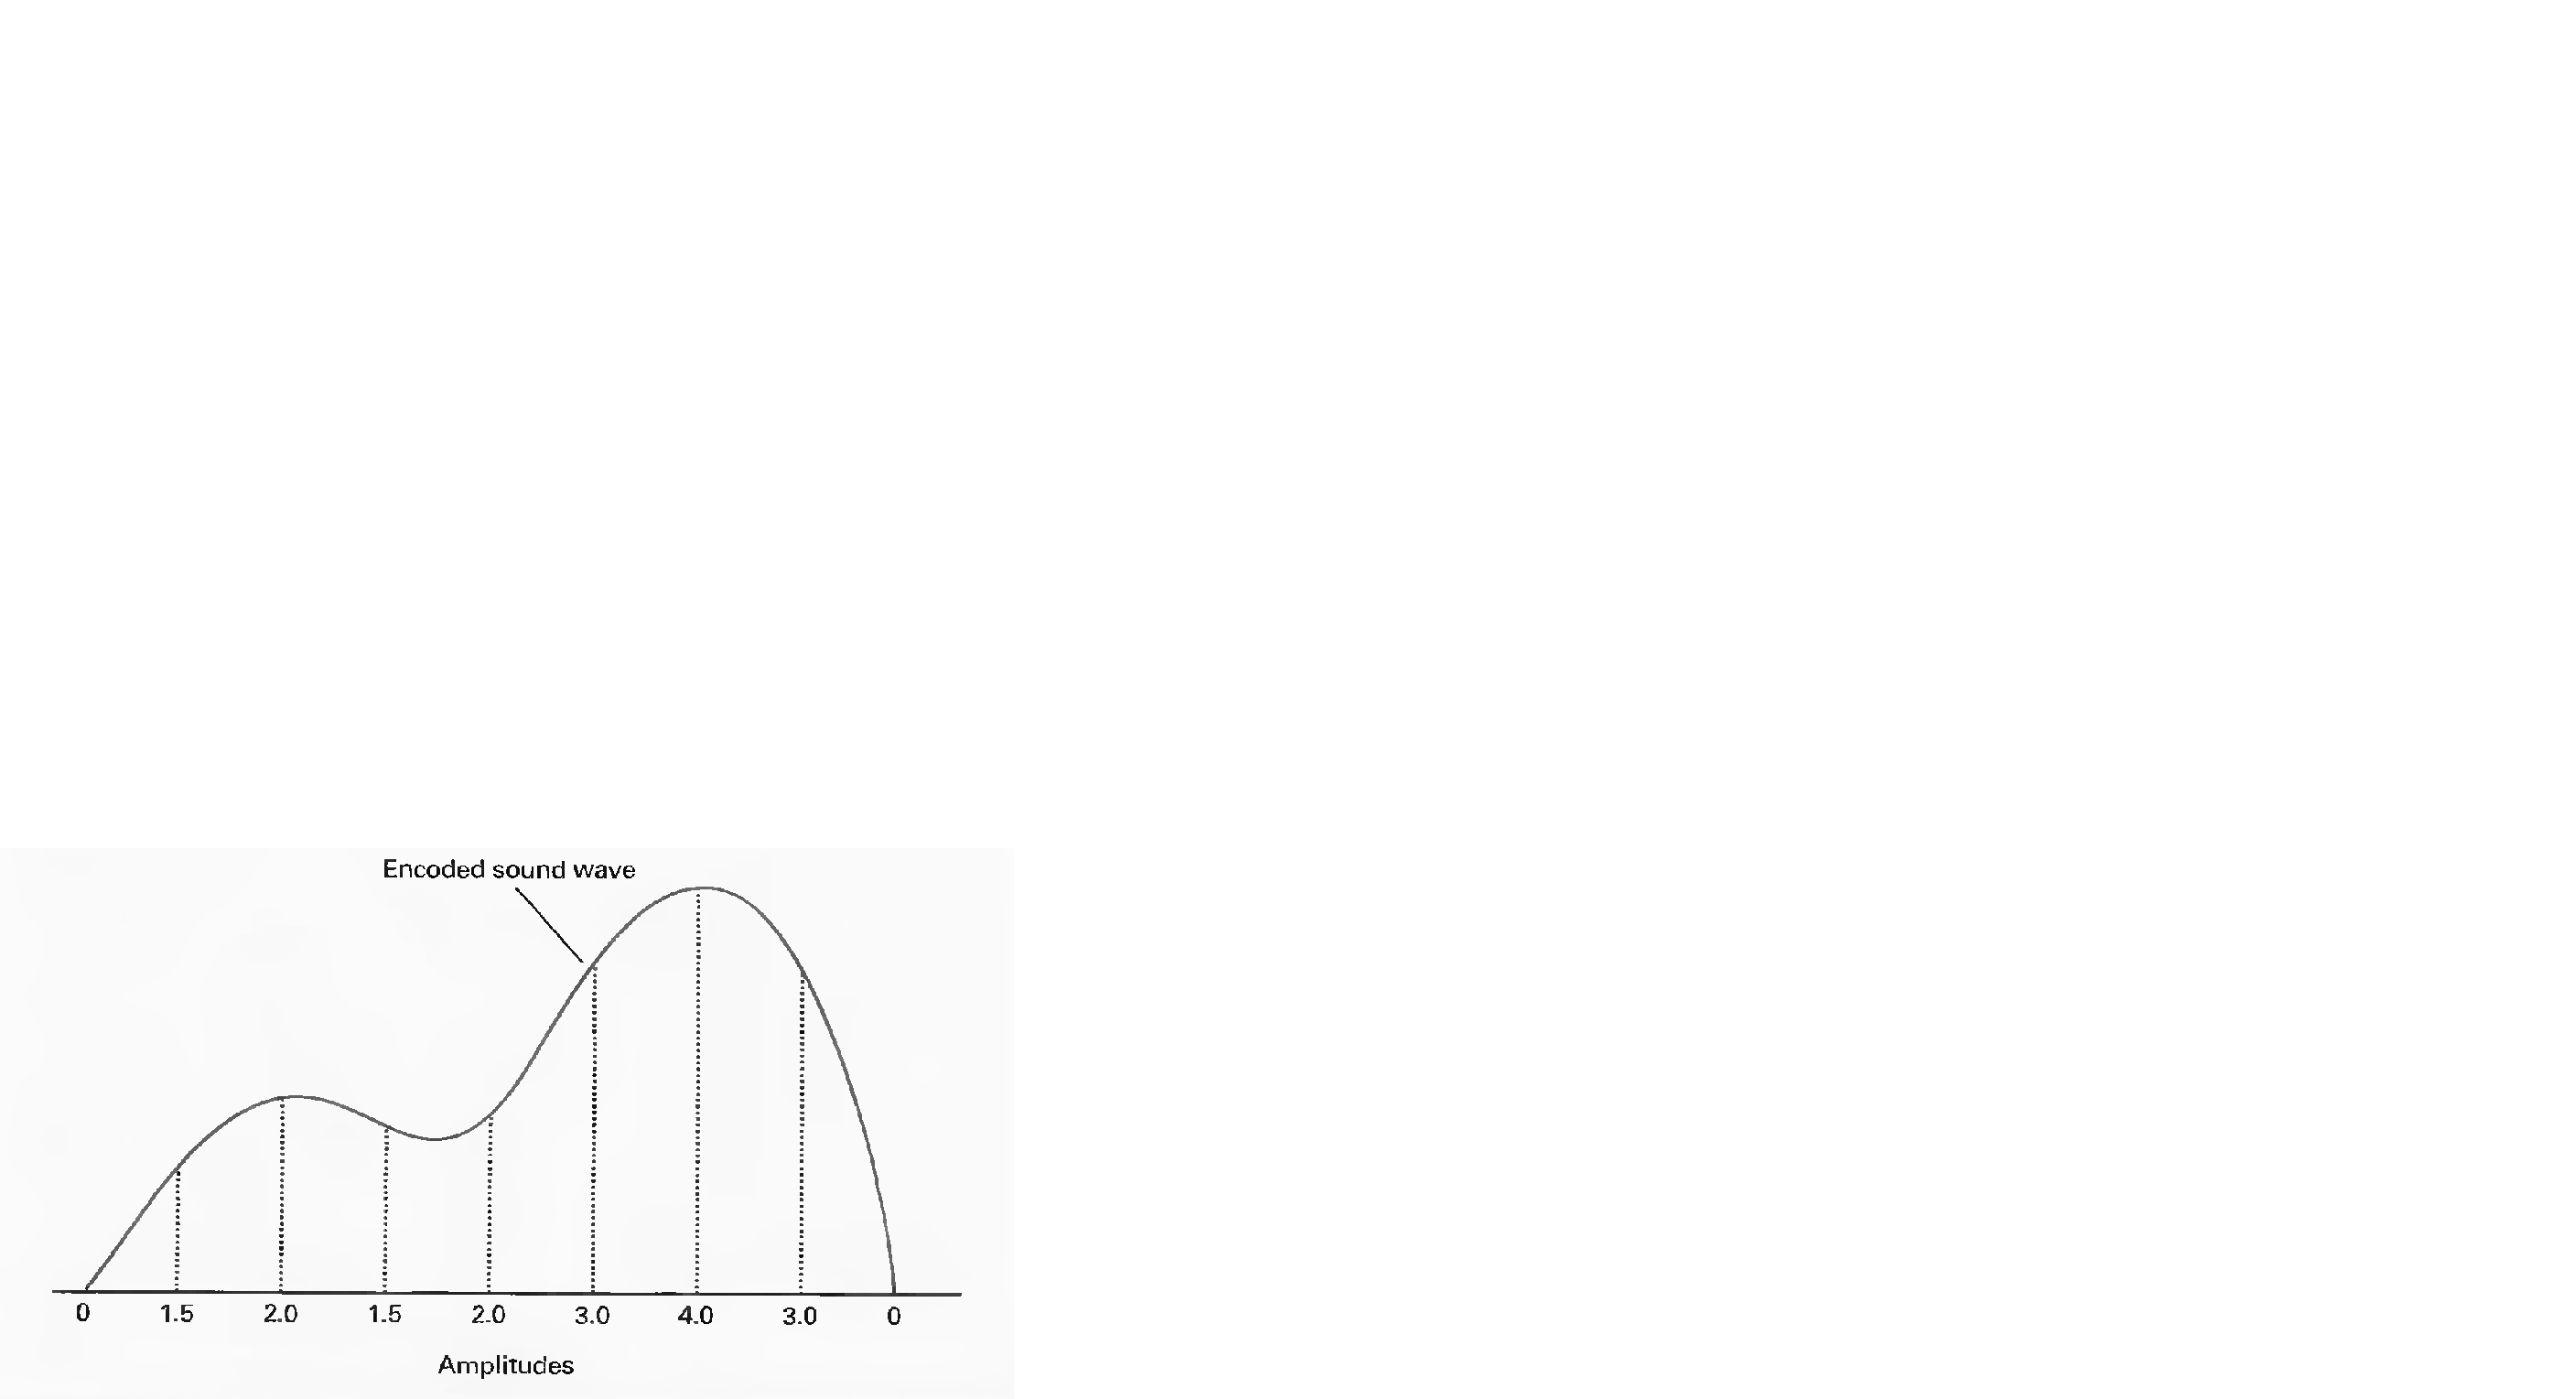
\includegraphics{ch2/Fig114.pdf}}
    \caption{Sóng âm được biểu diễn bởi dãy $0$, $1.5$, $2.0$, $3.0$, $4.0$, $3.0$, $0$}
  \label{fig:fig1.14}
\end{figure}


Một hệ thống mã hoá khác là Musical Instrumental Digital Interface (MIDI) được sử dụng
rộng rãi được sử dụng trong các bộ tổng hợp được tìm thấy trong các bàn phím điện tử,
trong âm thanh của các trò chơi video, và trong âm thanh hiệu ứng kèm các các trang
web. Bằng cách mã hoá các chỉ dẫn để tạo ra âm cho một thiết bị tổng hợp thay vì phải mã
hoá bản thân âm thanh, MIDI tránh được các yêu cầu lưu trữ lớn của kỹ thuật lấy mẫu. Chính
xác hơn, MIDI mã hoá các nốt nhạc của các nhạc cụ theo thời gian, ví dụ clarinet chơi nốt
Rê trong hai giây có thể mã hoá bằng ba byte thay vì mất hơn hai triệu bít bằng cách lấy
mẫu với tỷ lệ $44,100$ mẫu trên giây.

Nói tóm lại, ta có thể nghĩ MIDI như cách mã hoá các bản nhạc đọc bởi người biểu diễn thay
vì chính bản thân việc trình diễn, và việc chơi một file MIDI có thể nghe rất khác trên
các thiết bị tổng hợp khác nhau.

\subsection*{Câu hỏi \& Bài tập}

\begin{enumerate}
\item Đây là một thông điệp được mã hoá ở dạng ASCII dùng tám bít cho mỗi ký hiệu. Thông
  điệp này ý nghĩa là gì? (Xem Phụ lục \ref{})

\begin{tabular}{cccccc}
  01000011 &01101111 &01101101 &01110000 &01110101 &01110100  \\
  01100101 &01110010 &00100000 &01010011 &01100011 &01101001  \\
  01100101 &01101110 &01100011 &01100101 & &
\end{tabular}


\item Hãy chỉ ra mối quan hệ giữa mã của ký tự hoa và ký tự thường của
  cùng một ký tự theo bảng mã ASCII.

\item Mã hoá các câu sau theo bảng mã ASCII.
  \begin{enumerate}
  \item Where are you?

  \item "How?" Cheryl asked.

  \item 2 + 3 = 5.
  \end{enumerate}

\item Hãy mô tả một thiết bị trong cuộc sống hàng ngày có thể ở một trong hai trạng thái,
  ví dụ như lá cờ cắm trên cột cờ có thể ở trạng thái được treo hay không treo. Gán ký
  hiệu $1$ tới một trong hai trạng thái này và $0$ cho trạng thái còn lại, và chỉ ra cách
  biểu diễn ASCII cho ký tự $b$ khi lưu trữ dùng kiểu bít này.

\item Chuyển mỗi biểu diễn nhị phân sau đây sang cơ số mười:

  \begin{inparaenum}
  \item $0101 $ \hspace{2cm}
  \item $1001 $ \hspace{2cm}
  \item $1011 $

  \item $0110 $ \hspace{2cm}
  \item $10000$ \hspace{2cm}
  \item $10010$
  \end{inparaenum}

\item Chuyển mỗi biểu diễn thập phân sau đây sang nhị phân:

  \begin{inparaenum}
  \item $6$ \hspace{2cm} 
  \item $13$ \hspace{2cm}
  \item $11$ \hspace{2cm}


  \item $18$ \hspace{2cm}
  \item $27$ \hspace{2cm}
  \item $4$
  \end{inparaenum}

\item Nếu mỗi chữ số được mã hoá bởi một byte theo ASCII thì giá trị số lớn nhất có thể
  được biểu diễn dùng ba bytes là bao nhiêu? cũng vẫn ba byte đó nếu ta dùng ký hiệu nhị
  phân thì giá trị số lớn nhất là bao nhiêu?

\item Một lựa chọn khác so với ký hiệu hexa để biểu diễn dãy bít là \textbf{ký hiệu thập
    phân ngăn cách bởi dấu chấm} trong đó mỗi byte biểu diễn bởi giá trị ở cơ sở $10$
  tương đương. byte biểu diễn một số ngăn cách bởi các dấu chấm. Ví dụ, $12.5$ biểu diễn
  xâu $0000110000000101$ (byte $00001100$ biểu diễn số $12$, và $00000101$ biểu diễn số
  $5$), và xâu $100010000001000000000111$ được biểu diễn số $136.16.7$. Hãy biểu diễn mỗi
  xâu bít sau đây theo ký hiệu thập phân ngăn cách bởi dấu chấm.

  \begin{inparaenum}[a.]
  \item $0000111100001111$ \hspace {3cm}
  \item $001100110000000010000000$

  \item $0000101010100000$
  \end{inparaenum}

\item Chỉ ra ưu điểm của cách biểu diễn ảnh dùng kỹ thuật vector so với các kỹ thuật
  bitmap? ưu điểm của kỹ thuật bipmap so với kỹ thuật vector?

\item Giả sử ta dùng kỹ thuật lấy mẫu với $44,100$ mẫu trong một giây để thu âm stereo một
  giờ âm nhạc giống như đã thảo luận ở trên. Hãy so sánh kích thước của phiên bản được mã
  hoá theo cách này với một đĩa CD.
\end{enumerate}


















%%% Local Variables: 
%%% mode: latex
%%% TeX-master: "../tindaicuong"
%%% End: 
